\documentclass[urlrm]{usmthesis}
%%%%%%%%%%%%%%%%%%%%%%%%%%%%%%%%%%%%%%%%%%%%%%%%%%%%%%%
% This is usmthesis.tex, Nov 27 2007.
% Created by Lim Lian Tze,
% Computer Aided Translation Unit,
% School of Computer Sciences, 
% Universiti Sains Malaysia, Penang, Malaysia.
%
% This is the "main" file for the thesis, 
% formatted according to the Guide to the 
% Preparation, Submission and Examination of
% Theses, published by IPS USM.
%%%%%%%%%%%%%%%%%%%%%%%%%%%%%%%%%%%%%%%%%%%%%%%%%%%%%%%

%% Example of loading other packages that you may require.
%% I'm loading the marvosym package so that I can produce a
%% smiley face with the command \Smiley.
%%\usepackage{marvosym}

%% Enter particulars about your thesis HERE
% Your Name
\author{Chong Chee Kang}
% English title of your thesis
\title{Electric Drive Optimisation}
% Malay title of your thesis
%%\titlems{Penulisan Tesis dengan LaTeX}
% Year submitted
\submityear{2012}
% Month submitted
\submitmonth{June}
%% Choose only 1 degree type! :-)
%\degreetype{Doctor of Philosphy}
\degreetype{Bachelor of Mechanical Engineering}


%%%%%%%%%%%%%%%%%%%%%%%%%%%%%%%%%%%%%%%%%%%%%%%%%%%%%%%
%  You can comment out the following line if you don't have a
% "List of Own Publications"
%%%%%%%%%%%%%%%%%%%%%%%%%%%%%%%%%%%%%%%%%%%%%%%%%%%%%%%
%\newcites{own}{List of Publications}

%%%%%%%%%%%%%%%%%%%%%%%%%%%%%%%%%%%%%%%%%%%%%%%%%%%%%%%
% Options for generating hyperlinks when using pdfLaTeX
%%%%%%%%%%%%%%%%%%%%%%%%%%%%%%%%%%%%%%%%%%%%%%%%%%%%%%%
%%\ifpdf
%%  \makeatletter
%%  \usepackage[pdftex,plainpages=false,hypertexnames=false,bookmarksnumbered,pdfpagelabels,%
%%    pdfauthor={\@author},pdftitle={\@title}]{hyperref}
%%  \makeatother
%%\else
%%  \usepackage[dvips,plainpages=false,bookmarksnumbered,breaklinks=true]{hyperref}
%%\fi

%%pdf bookmark
\usepackage[pdftex,bookmarks=true]{hyperref}

%%%%%%%%%%%%%%%%%%%%%%%%%%%%%%%%%%%%%%%%%%%%%%%%%%%%%%%
% As we have loaded the natbib package, you can customise
% the citation style to some extent.  The following line
% specifies some standard punctuations:
%
% \bibpunct{#1}{#2}{#3}{#4}{#5}{#6}
% #1: open punctuation (a round bracket here)
% #2: close punctuation (a round bracket here)
% #3: punctuation separating multiple authors (a semi-colon here)
% #4: n - citation using numerical system
%     s - numeric superscript system
%     any other letter - author-year system
% #5: punctuation separating author name(s) from year
% #6: punctuation separating years for multiple citations
%     with same author(s)
%
% The default citation that I used here is therefore of the form
% (Wilks and Stevenson, 1999; Somers, 2000)
%
% You may change any of the 6 parameters if you prefer a
% different citation style.  Also see the natbib documentation.
%%%%%%%%%%%%%%%%%%%%%%%%%%%%%%%%%%%%%%%%%%%%%%%%%%%%%%%
\bibpunct{(}{)}{;}{a}{,}{,}
\begin{document}

%%%%%%%%%%%%%%%%%%%%%%%%%%%%%%%%%%%%%%%%%%%%%%%%%%%%%%%
% You can choose from several bibliography styles. I'm using
% the author-year system with agsm for the bibliography
% entries here, but feel free to experiment with other styles.
%
% If you prefer the number system though, use bibliography
% style "plainnat" for [1][2][3] or "alpha" for [Jon94] (the label
% will be auto-generated).
%%%%%%%%%%%%%%%%%%%%%%%%%%%%%%%%%%%%%%%%%%%%%%%%%%%%%%%
%\bibliographystyle{dcu}
%\bibliographystyleown{dcu}
\bibliographystyle{plainnat}
%\bibliographystyleown{plainnat}


\lstset{fontadjust=true}

\frontmatter

\addtocontents{lof}{\protect\raggedright\protect\sloppy}
\addtocontents{lof}{\protect\hfill{\protect\bfseries Page}\\}
\addtocontents{lot}{\protect\raggedright\protect\sloppy}
\addtocontents{lot}{\protect\hfill{\protect\bfseries Page}\\}

%%%%%%%%%%%%%%%%%%%%%%%%%%%%%%%%%%%%%%%%%%%%%%%%%%%%%%%
% Inserts the cover page (the hard cover with gold-lettering)
% and the title page 
%%%%%%%%%%%%%%%%%%%%%%%%%%%%%%%%%%%%%%%%%%%%%%%%%%%%%%%
\makecover


%%%%%%%%%%%%%%%%%%%%%%%%%%%%%%%%%%%%%%%%%%%%%%%%%%%%%%%
% Inserts a "Front Matter" bookmark if using pdfLaTeX
%%%%%%%%%%%%%%%%%%%%%%%%%%%%%%%%%%%%%%%%%%%%%%%%%%%%%%%
%%\ifpdf
%%    \pdfbookmark[-1]{Front Matter}{front}
%%\else\fi

%%%%%%%%%%%%%%%%%%%%%%%%%%%%%%%%%%%%%%%%%%%%%%%%%%%%%%%
% MAKE SURE YOU HAVE A acknowledgements.tex FILE
%%%%%%%%%%%%%%%%%%%%%%%%%%%%%%%%%%%%%%%%%%%%%%%%%%%%%%%
\chapter{Acknowledgements}




\renewcommand\contentsname{Table of Contents}
\begin{singlespace}
\tableofcontents \clearpage
\listoftables \clearpage
\listoffigures \clearpage
\end{singlespace}

%%%%%%%%%%%%%%%%%%%%%%%%%%%%%%%%%%%%%%%%%%%%%%%%%%%%%%%
% You can comment out the following line if you don't
% have a "List of Acronyms"
%%%%%%%%%%%%%%%%%%%%%%%%%%%%%%%%%%%%%%%%%%%%%%%%%%%%%%%
\chapter{List of Abbreviations}

\begin{acronym}[PMBLDC] %% replace 'MMMM' with the longest acronym in your list
\acro{AC}{Alternating Current}
\acro{DC}{Direct Current}
\acro{PMBLDC}{Permanent Magnet Brushless DC}
\acro{PWM}{Pulse Width Modulation}
\end{acronym}


\chapter{List of Symbols}

\begin{acronym}[lim ]
\acro{lim}[$\lim{}$]{limit}
\end{acronym}



% Paragraph spacing
\setlength\parskip{18pt}
% Text-float spacing
\setlength\intextsep{24pt}

%%%%%%%%%%%%%%%%%%%%%%%%%%%%%%%%%%%%%%%%%%%%%%%%%%%%%%%
% Your Malay and English abstracts, each in one file.
%%%%%%%%%%%%%%%%%%%%%%%%%%%%%%%%%%%%%%%%%%%%%%%%%%%%%%%
\begin{MsAbstract}
Abstrak versi bahasa melayu
\end{MsAbstract}

\begin{EnAbstract}
English version of the abstract
\end{EnAbstract}


\addtocontents{toc}{\protect\setlength{\protect\cftbeforechapskip}{2.5pc}}
\addtocontents{toc}{\protect\cftpagenumbersoff{chap}}
 
\mainmatter
%%\ifpdf
%%  \pdfbookmark[-1]{Main Chapters}{main}
%%\else\fi

%%%%%%%%%%%%%%%%%%%%%%%%%%%%%%%%%%%%%%%%%%%%%%%%%%%%%%%
% The actual chapters of your thesis as listed in 
% mainchaps.tex. Make sure you have the relevant
% chapter files. 
% E.g. if you mainchaps.tex contains the lines
%
%  \include{hypothesis.tex}
%  \include{proof.tex}
%
% Then you MUST have the files hypothesis.tex, proof.tex
% (containing the relevant chapters) in the same directory
% as mainchaps.tex.
%%%%%%%%%%%%%%%%%%%%%%%%%%%%%%%%%%%%%%%%%%%%%%%%%%%%%%%
\chapter{Introduction}\label{chap:intro}
\section{Background}

Electric motor can be classified into two major categories which are the DC electric motor and AC electric motor. An AC motor is an electric motor driven by alternating current whereas a DC motor is driven by direct current. There are various types of AC motor which includes induction motor, synchronous motor, eddy current motor and etc. The DC electric motor includes permanent magnet brushed motor, permanent magnet brushless motor, switched reluctance motor and etc.

Electric motor is used in many application which includes in machine for driving the pulley and belts, the conveyor belt, in drilling and lathe machine. Apart from the heavy industry, electric motor is used in home appliances for powering the washing machine, fan, blower of air-conditioner and blender machine. Moreover, electric motor is also used in automobile industry as the starter motor for firing up the internal combustion engine of cars and trucks and last but not least, as the drive train for electric vehicle.

The PMBLDC is a synchronous motor. In other words, the frequency of the magnetic field generated at the stator and the rotor is the same. PMBLDC comes in single-phase, 2-phase and 3-phase configuration which the 3-phase configuration is the most popular among the three. There are basically two major components inside a PMBLDC motor which is the stator and the rotor. The stator of a PMBLDC motor is made up of 
a series of laminated steel with wire windings around it. The rotor is build up of permanent magnet that has at least 2 poles.

Unlike brushed motor, PMBLDC does not have brushes for comutation, instead a controller is needed for controlling the rotation of the PMBLDC by sending out AC signal to the PMBLDC. There are two types of AC signal sent to the PMBLDC for controlling the motor which are the Trapezoidal type and the Sinusoidal type which depends on the winding of the stator.

In order for the controller to send out the correct signal, the position of the rotor must be sent to the controller so that a sequence of AC signal can be generated which energized the winding of the stator for rotating the motor. Hall effect sensors is used as the rotor position detection sensor which has an analog signal output. When the magnetic field is detected by the hall effect sensor, the voltage output will be changes from lowest to the highest or vice versa depending on the circuit configuration. Normally there are three hall effect sensor mounted on the stator of PMBLDC motor which are 60\textdegree or 120\textdegree apart depending on the number of poles and the comutation sequence required.

Figure 1.1 shows the hall effect sensors signal for a 2 pole PMBLDC motor, the back emf, the phase current and the output torque. As shown in the figure, there are 3 hall effect sensors with labels A, B and C respectively, sensor A is leading sensor B by 60\textdegree and sensor B is leading sensor C by 60\textdegree. 

%%The back EMF is generated by each of it's stator winding when the motor is rotating which has an opposite direction to the supply voltage which agrees to Lenz's law stating that "An induced electromotive force always give rise to a current whose magnetic field opposes the original change in magnetic flux". Therefore, from figure 1.1, it can ......

Ideally, the phase current should behave as a digital square wave signal where the current rises and drops immediately. But in real world, the current would take some time to rises from zero to maximum/minimum. Hence, the torque produced would behave as a series of ripple instead of a constant output torque.

\begin{figure}
	\centering
	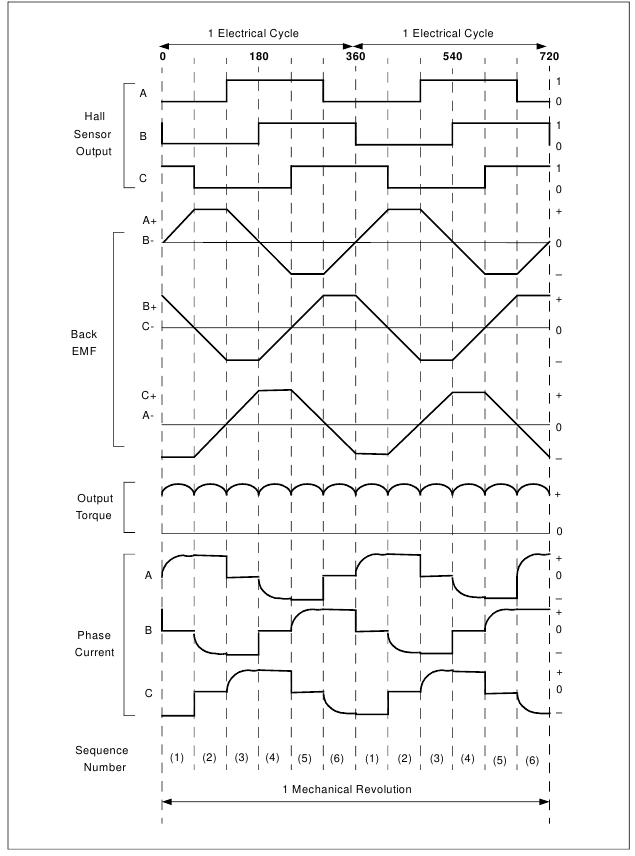
\includegraphics[width=5.5in]{images/signal.jpg}
	\caption{Hall effect sensors signal, back emf, output torque and phase current \citep{an885}}
\end{figure}

In this project, a PMBLDC hub motor is used as the sole powertrain of a electric vehicle. The electric vehicle will be used for participating the Shell Eco-Marathon which is a competition which teams compete to build a higher mileage vehicle. The competition requires the participating teams to build their own car for the categories they are participating( for example, the urban concept category or the prototype category). For our case, a four-wheel electric vehicle is built for participation in urban concept category. The vehicle will be driven around a race track, which is the Sepang Internation Track, North Track for year 2012 for four laps with 10 seconds of stop between each lap. The energy consumption will be collected and the mileage will be calculated for each attempt and every team will have 3 attempts for mileage improvement.

\section{Problem Statement}
PMBLDC motor is better compare to brushed DC motor because brushless motor increases the efficiency by dropping the friction between the brush and the comutator which happens in brushed DC motor. However, the inefficient PWM in controlling the speed of the motor and the torque ripple cause by the phase current limits the efficiency of a PMBLDC motor.

There are three types of torque produced by a permanent magnet electric motor which are:

\begin{itemize}
	\item cogging torque
	\item reluctance torque
	\item mutual torque
\end{itemize}

The cogging torque is produced by the interaction between the permanent magnet at the rotor and the stator slots. Cogging torque is an undesireable torque generated by the electric motor which dominates at low speed and results in speed ripple. Cogging torque can only be minimize by means of hardware tuning which includes altering the number of poles, teeth at the stator or editing the controller setting which changes the drive current waveform.

The reluctance torque is generated by the difference in position of the rotor and the phase induction at the rotor. The ripple produced by the reluctance torque could be negligible with a good number of poles and slots of the windings at the stator.

The third type of torque produced by PMBLDC motor is the mutual torque which is caused by the non-sinusoidal signal reaching the stator windings or the magnet at the rotor. Since the torque is generated by the current, ripple reduction for mutual torque could be achieved by fine-tuning the current signal.

The torque ripple occurs in PMBLDC is mainly contributed by the different rise and decay time of the phase current as shown in figure 1.1. The cogging torque does contribute to torque ripple in low speed but it's negligible at high speed. Torque ripple contributed by reluctance torque could also be ignored since the high number of poles and stator slot minimize the ripple. Mutual torque would be the major contributor to torque ripple due to the direct dependency on the current.

Based on figure 1.2 (a), the rate of decay of $i_a$ is faster than the rate of increase of $i_b$. Therefore, at certain point where $i_a$ reaches 0 but $i_b$ 

\begin{figure}[htb]
	\centering
	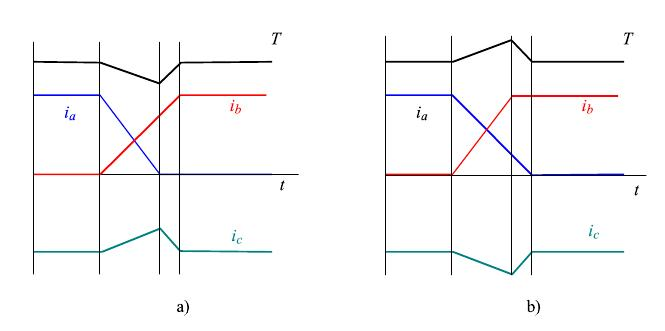
\includegraphics[width=5.5in]{images/phase_current.jpg}
	\caption{The phase current and torque during an alternating comutation event  \citep{7648}}
\end{figure}

%%Due to the PMBLDC and the controller used in the project is proprietary and sponsored, the modification to the electric motor structure which includes the rotor poles, stator winding, hall effect sensors within the PMBLDC motor and the controller's wiring and signal input/output is impossible. 



\chapter{Literature Review}\label{chap:literature}

\chapter{Methodology}\label{chap:methodology}

\chapter{Result and Discussion}

\chapter{Conclusion}




\addtocontents{toc}{\protect\cftpagenumberson{chap}}

%%\ifpdf
%%  \pdfbookmark[-1]{Back Matter}{back}
%%\else\fi

\begin{singlespace}
%%%%%%%%%%%%%%%%%%%%%%%%%%%%%%%%%%%%%%%%%%%%%%%%%%%%%%%
% The bibliography.
% You can create mybib.bib with JabRef, the program included
% in the Colloquium05 CD-ROM.  Or download from
% http://jabref.sourceforge.net/
%%%%%%%%%%%%%%%%%%%%%%%%%%%%%%%%%%%%%%%%%%%%%%%%%%%%%%%
\bibliography{mybib}
\end{singlespace}

\addtocontents{toc}{\protect\setlength{\protect\cftbeforechapskip}{1pc}}


%%%%%%%%%%%%%%%%%%%%%%%%%%%%%%%%%%%%%%%%%%%%%%%%%%%%%%%
% The appendices.
% If you don't have any, you may delete everything below,
% until and including \chapter{Schematic}


.
%%%%%%%%%%%%%%%%%%%%%%%%%%%%%%%%%%%%%%%%%%%%%%%%%%%%%%%
\clearpage
\appendix
\phantomsection\addcontentsline{toc}{part}{\texorpdfstring{\uppercase{Appendices}}{Appendices}}
\thispagestyle{empty}
\vspace*{\stretch{1}}
  \begin{center}
    {\Huge\bfseries APPENDICES}
  \end{center}
\vspace*{\stretch{2}}
\addtocontents{toc}{\protect\renewcommand{\protect\chaptername}{\appendixname}} 
\addtocontents{toc}{\protect\setlength\cftchapnumwidth{7pc}}

\renewcommand\chaptername{\appendixname}
\chapter{Schematic}




%%%%%%%%%%%%%%%%%%%%%%%%%%%%%%%%%%%%%%%%%%%%%%%%%%%%%%%
% The list of own publications.  If you don't have one, you may
% comment out the next 3 lines (up till just before \end{singlespace}.
%%%%%%%%%%%%%%%%%%%%%%%%%%%%%%%%%%%%%%%%%%%%%%%%%%%%%%%
%%\nociteown{lim:2007,lim:latextypesetting}
%%\addtocontents{toc}{\protect\setlength{\protect\cftbeforechapskip}{3pc}}
%%\begin{singlespace}
%%\bibliographyown{mybib}
%%\end{singlespace}

\end{document}
